% Figure 3: Phase 3 cumulative reconstruction curve
% Line chart showing score as traits are added in tier order.
% Pass region (y>=33) shaded green; fail region (y<33) shaded red.
% Self-contained figure environment — requires pgfplots, xcolor, tikz.
%
% Usage in main.tex:  % Figure 3: Phase 3 cumulative reconstruction curve
% Line chart showing score as traits are added in tier order.
% Pass region (y>=33) shaded green; fail region (y<33) shaded red.
% Self-contained figure environment — requires pgfplots, xcolor, tikz.
%
% Usage in main.tex:  % Figure 3: Phase 3 cumulative reconstruction curve
% Line chart showing score as traits are added in tier order.
% Pass region (y>=33) shaded green; fail region (y<33) shaded red.
% Self-contained figure environment — requires pgfplots, xcolor, tikz.
%
% Usage in main.tex:  % Figure 3: Phase 3 cumulative reconstruction curve
% Line chart showing score as traits are added in tier order.
% Pass region (y>=33) shaded green; fail region (y<33) shaded red.
% Self-contained figure environment — requires pgfplots, xcolor, tikz.
%
% Usage in main.tex:  \input{figures/fig3-reconstruction}

\begin{figure}[tbp]
\centering
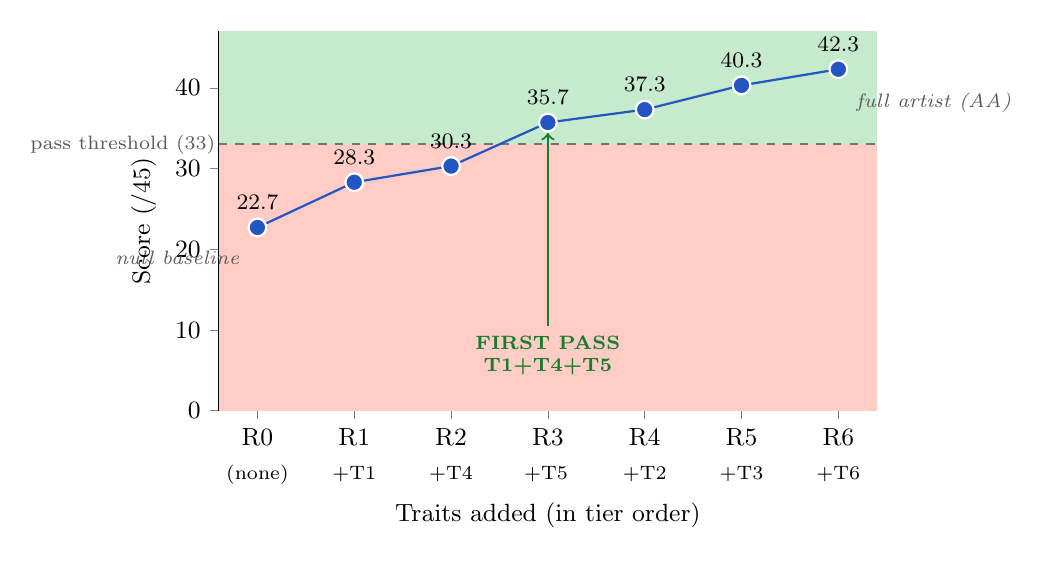
\begin{tikzpicture}
\begin{axis}[
  width=0.82\linewidth,
  height=6.4cm,
  xmin=-0.4, xmax=6.4,
  ymin=0, ymax=47,
  xlabel={Traits added (in tier order)},
  xlabel style={font=\small},
  ylabel={Score (/45)},
  ylabel style={font=\small},
  xtick={0,1,2,3,4,5,6},
  xticklabels={
    R0\\[0.3ex]{\scriptsize(none)},
    R1\\[0.3ex]{\scriptsize$+$T1},
    R2\\[0.3ex]{\scriptsize$+$T4},
    R3\\[0.3ex]{\scriptsize$+$T5\,$\bigstar$},
    R4\\[0.3ex]{\scriptsize$+$T2},
    R5\\[0.3ex]{\scriptsize$+$T3},
    R6\\[0.3ex]{\scriptsize$+$T6}
  },
  xticklabel style={font=\small, align=center},
  ytick={0,10,20,30,40},
  yticklabel style={font=\small},
  tick align=outside,
  major tick length=3pt,
  axis line style={thin},
  axis lines*=left,
  clip=false,
  enlargelimits=false,
]

  %% -------------------------------------------------------
  %% Background: FAIL region  (0 <= y <= 33), drawn as filled rectangle
  %% Use \fill in tikz coordinate space via axis cs
  %% -------------------------------------------------------
  \fill[
    fill={rgb,255:red,255;green,205;blue,198},
    draw=none,
  ]
    (axis cs:-0.4, 0) rectangle (axis cs:6.4, 33);

  %% -------------------------------------------------------
  %% Background: PASS region  (33 <= y <= 47)
  %% -------------------------------------------------------
  \fill[
    fill={rgb,255:red,198;green,235;blue,204},
    draw=none,
  ]
    (axis cs:-0.4, 33) rectangle (axis cs:6.4, 47);

  %% -------------------------------------------------------
  %% Pass threshold dashed horizontal line at y=33
  %% -------------------------------------------------------
  \addplot[
    color=black!55,
    dashed,
    thick,
    mark=none,
    forget plot,
  ] coordinates { (-0.4, 33) (6.4, 33) };

  \node[
    font=\scriptsize,
    anchor=east,
    text=black!65,
    fill=white,
    inner sep=1pt,
  ] at (axis cs: -0.4, 33) {pass threshold (33)};

  %% -------------------------------------------------------
  %% Reconstruction line: blue, filled circle markers
  %% -------------------------------------------------------
  \addplot[
    color={rgb,255:red,35;green,85;blue,195},
    thick,
    mark=*,
    mark size=3.2pt,
    mark options={
      fill={rgb,255:red,35;green,85;blue,195},
      draw=white,
      line width=0.8pt,
    },
    forget plot,
  ] coordinates {
    (0, 22.7)   % R0  null baseline
    (1, 28.3)   % R1  +T1
    (2, 30.3)   % R2  +T4
    (3, 35.7)   % R3  first pass  *** FIRST PASS ***
    (4, 37.3)   % R4  +T2
    (5, 40.3)   % R5  +T3
    (6, 42.3)   % R6  full artist
  };

  %% -------------------------------------------------------
  %% Score labels above each data point
  %% -------------------------------------------------------
  \node[font=\footnotesize, anchor=south, yshift=3pt]
    at (axis cs: 0, 22.7) {22.7};
  \node[font=\footnotesize, anchor=south, yshift=3pt]
    at (axis cs: 1, 28.3) {28.3};
  \node[font=\footnotesize, anchor=south, yshift=3pt]
    at (axis cs: 2, 30.3) {30.3};
  \node[font=\footnotesize, anchor=south, yshift=3pt]
    at (axis cs: 3, 35.7) {35.7};
  \node[font=\footnotesize, anchor=south, yshift=3pt]
    at (axis cs: 4, 37.3) {37.3};
  \node[font=\footnotesize, anchor=south, yshift=3pt]
    at (axis cs: 5, 40.3) {40.3};
  \node[font=\footnotesize, anchor=south, yshift=3pt]
    at (axis cs: 6, 42.3) {42.3};

  %% -------------------------------------------------------
  %% Annotation: "null baseline" at R0
  %% -------------------------------------------------------
  \node[
    font=\scriptsize\itshape,
    anchor=north east,
    text=black!65,
    xshift=-3pt,
    yshift=-5pt,
  ] at (axis cs: 0, 22.7) {null baseline};

  %% -------------------------------------------------------
  %% Annotation: "full artist (AA)" at R6
  %% -------------------------------------------------------
  \node[
    font=\scriptsize\itshape,
    anchor=north west,
    text=black!65,
    xshift=3pt,
    yshift=-5pt,
  ] at (axis cs: 6, 42.3) {full artist (AA)};

  %% -------------------------------------------------------
  %% Annotation: "FIRST PASS — T1+T4+T5" at R3
  %% Upward arrow from y=10 to just below the R3 data point
  %% -------------------------------------------------------
  \draw[
    ->,
    thick,
    color={rgb,255:red,25;green,125;blue,45},
  ] (axis cs: 3, 10.5) -- (axis cs: 3, 34.4);

  \node[
    font=\scriptsize\bfseries,
    anchor=north,
    text={rgb,255:red,25;green,125;blue,45},
    align=center,
    inner sep=2pt,
  ] at (axis cs: 3, 10.0) {FIRST PASS\\T1+T4+T5};

\end{axis}
\end{tikzpicture}

\caption{Reconstruction curve (Phase~3): cumulative score as traits are added
  in tier order. The quality threshold is first crossed at R3
  (T1+T4+T5 = 35.7/45, $\bigstar$). Each subsequent trait adds
  1.6--5.4 points. The minimum sufficient set is T1 + T4 + T5.}
\label{fig:reconstruction}
\end{figure}


\begin{figure}[tbp]
\centering
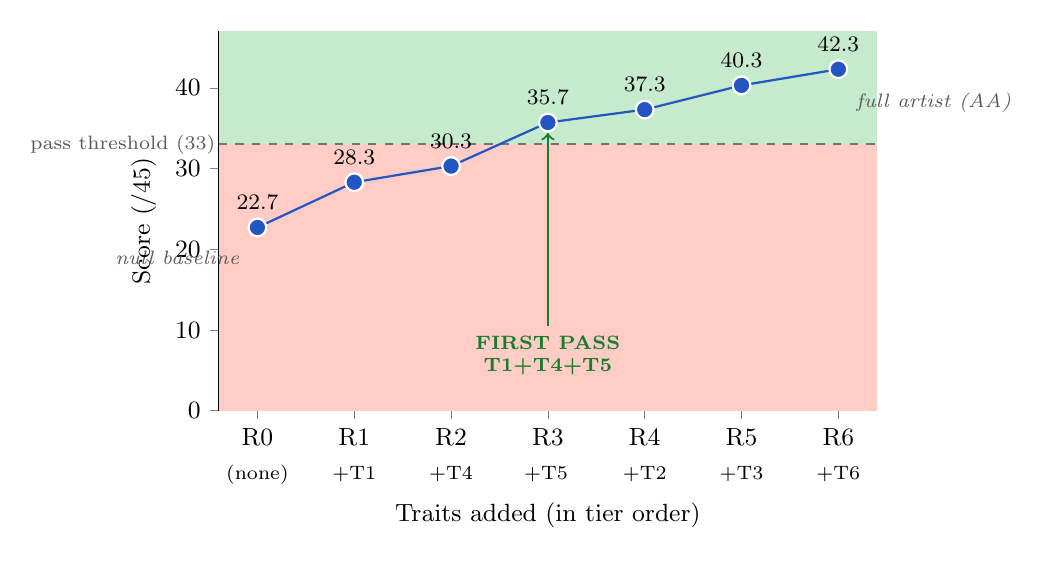
\begin{tikzpicture}
\begin{axis}[
  width=0.82\linewidth,
  height=6.4cm,
  xmin=-0.4, xmax=6.4,
  ymin=0, ymax=47,
  xlabel={Traits added (in tier order)},
  xlabel style={font=\small},
  ylabel={Score (/45)},
  ylabel style={font=\small},
  xtick={0,1,2,3,4,5,6},
  xticklabels={
    R0\\[0.3ex]{\scriptsize(none)},
    R1\\[0.3ex]{\scriptsize$+$T1},
    R2\\[0.3ex]{\scriptsize$+$T4},
    R3\\[0.3ex]{\scriptsize$+$T5\,$\bigstar$},
    R4\\[0.3ex]{\scriptsize$+$T2},
    R5\\[0.3ex]{\scriptsize$+$T3},
    R6\\[0.3ex]{\scriptsize$+$T6}
  },
  xticklabel style={font=\small, align=center},
  ytick={0,10,20,30,40},
  yticklabel style={font=\small},
  tick align=outside,
  major tick length=3pt,
  axis line style={thin},
  axis lines*=left,
  clip=false,
  enlargelimits=false,
]

  %% -------------------------------------------------------
  %% Background: FAIL region  (0 <= y <= 33), drawn as filled rectangle
  %% Use \fill in tikz coordinate space via axis cs
  %% -------------------------------------------------------
  \fill[
    fill={rgb,255:red,255;green,205;blue,198},
    draw=none,
  ]
    (axis cs:-0.4, 0) rectangle (axis cs:6.4, 33);

  %% -------------------------------------------------------
  %% Background: PASS region  (33 <= y <= 47)
  %% -------------------------------------------------------
  \fill[
    fill={rgb,255:red,198;green,235;blue,204},
    draw=none,
  ]
    (axis cs:-0.4, 33) rectangle (axis cs:6.4, 47);

  %% -------------------------------------------------------
  %% Pass threshold dashed horizontal line at y=33
  %% -------------------------------------------------------
  \addplot[
    color=black!55,
    dashed,
    thick,
    mark=none,
    forget plot,
  ] coordinates { (-0.4, 33) (6.4, 33) };

  \node[
    font=\scriptsize,
    anchor=east,
    text=black!65,
    fill=white,
    inner sep=1pt,
  ] at (axis cs: -0.4, 33) {pass threshold (33)};

  %% -------------------------------------------------------
  %% Reconstruction line: blue, filled circle markers
  %% -------------------------------------------------------
  \addplot[
    color={rgb,255:red,35;green,85;blue,195},
    thick,
    mark=*,
    mark size=3.2pt,
    mark options={
      fill={rgb,255:red,35;green,85;blue,195},
      draw=white,
      line width=0.8pt,
    },
    forget plot,
  ] coordinates {
    (0, 22.7)   % R0  null baseline
    (1, 28.3)   % R1  +T1
    (2, 30.3)   % R2  +T4
    (3, 35.7)   % R3  first pass  *** FIRST PASS ***
    (4, 37.3)   % R4  +T2
    (5, 40.3)   % R5  +T3
    (6, 42.3)   % R6  full artist
  };

  %% -------------------------------------------------------
  %% Score labels above each data point
  %% -------------------------------------------------------
  \node[font=\footnotesize, anchor=south, yshift=3pt]
    at (axis cs: 0, 22.7) {22.7};
  \node[font=\footnotesize, anchor=south, yshift=3pt]
    at (axis cs: 1, 28.3) {28.3};
  \node[font=\footnotesize, anchor=south, yshift=3pt]
    at (axis cs: 2, 30.3) {30.3};
  \node[font=\footnotesize, anchor=south, yshift=3pt]
    at (axis cs: 3, 35.7) {35.7};
  \node[font=\footnotesize, anchor=south, yshift=3pt]
    at (axis cs: 4, 37.3) {37.3};
  \node[font=\footnotesize, anchor=south, yshift=3pt]
    at (axis cs: 5, 40.3) {40.3};
  \node[font=\footnotesize, anchor=south, yshift=3pt]
    at (axis cs: 6, 42.3) {42.3};

  %% -------------------------------------------------------
  %% Annotation: "null baseline" at R0
  %% -------------------------------------------------------
  \node[
    font=\scriptsize\itshape,
    anchor=north east,
    text=black!65,
    xshift=-3pt,
    yshift=-5pt,
  ] at (axis cs: 0, 22.7) {null baseline};

  %% -------------------------------------------------------
  %% Annotation: "full artist (AA)" at R6
  %% -------------------------------------------------------
  \node[
    font=\scriptsize\itshape,
    anchor=north west,
    text=black!65,
    xshift=3pt,
    yshift=-5pt,
  ] at (axis cs: 6, 42.3) {full artist (AA)};

  %% -------------------------------------------------------
  %% Annotation: "FIRST PASS — T1+T4+T5" at R3
  %% Upward arrow from y=10 to just below the R3 data point
  %% -------------------------------------------------------
  \draw[
    ->,
    thick,
    color={rgb,255:red,25;green,125;blue,45},
  ] (axis cs: 3, 10.5) -- (axis cs: 3, 34.4);

  \node[
    font=\scriptsize\bfseries,
    anchor=north,
    text={rgb,255:red,25;green,125;blue,45},
    align=center,
    inner sep=2pt,
  ] at (axis cs: 3, 10.0) {FIRST PASS\\T1+T4+T5};

\end{axis}
\end{tikzpicture}

\caption{Reconstruction curve (Phase~3): cumulative score as traits are added
  in tier order. The quality threshold is first crossed at R3
  (T1+T4+T5 = 35.7/45, $\bigstar$). Each subsequent trait adds
  1.6--5.4 points. The minimum sufficient set is T1 + T4 + T5.}
\label{fig:reconstruction}
\end{figure}


\begin{figure}[tbp]
\centering
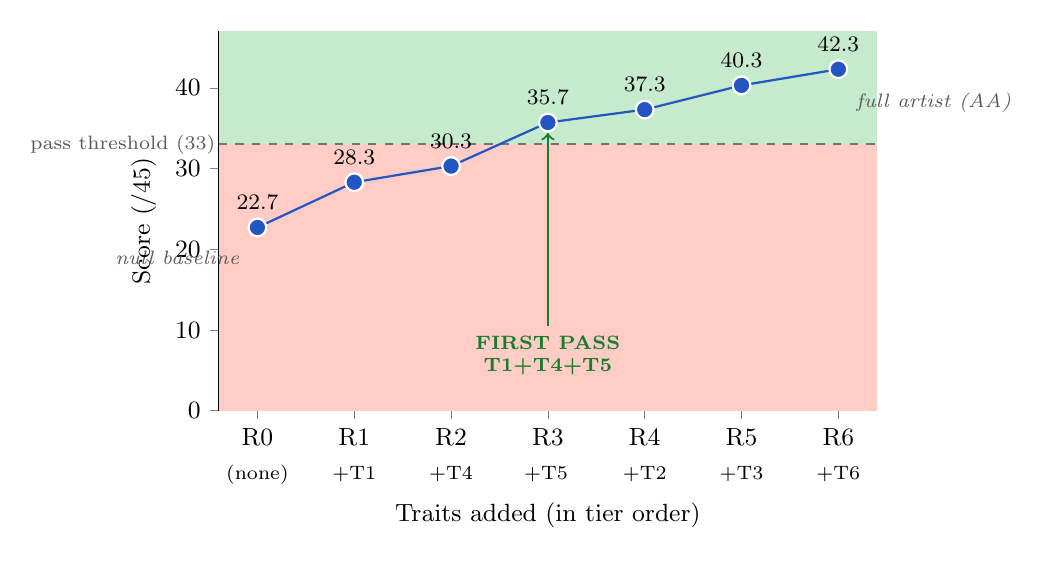
\begin{tikzpicture}
\begin{axis}[
  width=0.82\linewidth,
  height=6.4cm,
  xmin=-0.4, xmax=6.4,
  ymin=0, ymax=47,
  xlabel={Traits added (in tier order)},
  xlabel style={font=\small},
  ylabel={Score (/45)},
  ylabel style={font=\small},
  xtick={0,1,2,3,4,5,6},
  xticklabels={
    R0\\[0.3ex]{\scriptsize(none)},
    R1\\[0.3ex]{\scriptsize$+$T1},
    R2\\[0.3ex]{\scriptsize$+$T4},
    R3\\[0.3ex]{\scriptsize$+$T5\,$\bigstar$},
    R4\\[0.3ex]{\scriptsize$+$T2},
    R5\\[0.3ex]{\scriptsize$+$T3},
    R6\\[0.3ex]{\scriptsize$+$T6}
  },
  xticklabel style={font=\small, align=center},
  ytick={0,10,20,30,40},
  yticklabel style={font=\small},
  tick align=outside,
  major tick length=3pt,
  axis line style={thin},
  axis lines*=left,
  clip=false,
  enlargelimits=false,
]

  %% -------------------------------------------------------
  %% Background: FAIL region  (0 <= y <= 33), drawn as filled rectangle
  %% Use \fill in tikz coordinate space via axis cs
  %% -------------------------------------------------------
  \fill[
    fill={rgb,255:red,255;green,205;blue,198},
    draw=none,
  ]
    (axis cs:-0.4, 0) rectangle (axis cs:6.4, 33);

  %% -------------------------------------------------------
  %% Background: PASS region  (33 <= y <= 47)
  %% -------------------------------------------------------
  \fill[
    fill={rgb,255:red,198;green,235;blue,204},
    draw=none,
  ]
    (axis cs:-0.4, 33) rectangle (axis cs:6.4, 47);

  %% -------------------------------------------------------
  %% Pass threshold dashed horizontal line at y=33
  %% -------------------------------------------------------
  \addplot[
    color=black!55,
    dashed,
    thick,
    mark=none,
    forget plot,
  ] coordinates { (-0.4, 33) (6.4, 33) };

  \node[
    font=\scriptsize,
    anchor=east,
    text=black!65,
    fill=white,
    inner sep=1pt,
  ] at (axis cs: -0.4, 33) {pass threshold (33)};

  %% -------------------------------------------------------
  %% Reconstruction line: blue, filled circle markers
  %% -------------------------------------------------------
  \addplot[
    color={rgb,255:red,35;green,85;blue,195},
    thick,
    mark=*,
    mark size=3.2pt,
    mark options={
      fill={rgb,255:red,35;green,85;blue,195},
      draw=white,
      line width=0.8pt,
    },
    forget plot,
  ] coordinates {
    (0, 22.7)   % R0  null baseline
    (1, 28.3)   % R1  +T1
    (2, 30.3)   % R2  +T4
    (3, 35.7)   % R3  first pass  *** FIRST PASS ***
    (4, 37.3)   % R4  +T2
    (5, 40.3)   % R5  +T3
    (6, 42.3)   % R6  full artist
  };

  %% -------------------------------------------------------
  %% Score labels above each data point
  %% -------------------------------------------------------
  \node[font=\footnotesize, anchor=south, yshift=3pt]
    at (axis cs: 0, 22.7) {22.7};
  \node[font=\footnotesize, anchor=south, yshift=3pt]
    at (axis cs: 1, 28.3) {28.3};
  \node[font=\footnotesize, anchor=south, yshift=3pt]
    at (axis cs: 2, 30.3) {30.3};
  \node[font=\footnotesize, anchor=south, yshift=3pt]
    at (axis cs: 3, 35.7) {35.7};
  \node[font=\footnotesize, anchor=south, yshift=3pt]
    at (axis cs: 4, 37.3) {37.3};
  \node[font=\footnotesize, anchor=south, yshift=3pt]
    at (axis cs: 5, 40.3) {40.3};
  \node[font=\footnotesize, anchor=south, yshift=3pt]
    at (axis cs: 6, 42.3) {42.3};

  %% -------------------------------------------------------
  %% Annotation: "null baseline" at R0
  %% -------------------------------------------------------
  \node[
    font=\scriptsize\itshape,
    anchor=north east,
    text=black!65,
    xshift=-3pt,
    yshift=-5pt,
  ] at (axis cs: 0, 22.7) {null baseline};

  %% -------------------------------------------------------
  %% Annotation: "full artist (AA)" at R6
  %% -------------------------------------------------------
  \node[
    font=\scriptsize\itshape,
    anchor=north west,
    text=black!65,
    xshift=3pt,
    yshift=-5pt,
  ] at (axis cs: 6, 42.3) {full artist (AA)};

  %% -------------------------------------------------------
  %% Annotation: "FIRST PASS — T1+T4+T5" at R3
  %% Upward arrow from y=10 to just below the R3 data point
  %% -------------------------------------------------------
  \draw[
    ->,
    thick,
    color={rgb,255:red,25;green,125;blue,45},
  ] (axis cs: 3, 10.5) -- (axis cs: 3, 34.4);

  \node[
    font=\scriptsize\bfseries,
    anchor=north,
    text={rgb,255:red,25;green,125;blue,45},
    align=center,
    inner sep=2pt,
  ] at (axis cs: 3, 10.0) {FIRST PASS\\T1+T4+T5};

\end{axis}
\end{tikzpicture}

\caption{Reconstruction curve (Phase~3): cumulative score as traits are added
  in tier order. The quality threshold is first crossed at R3
  (T1+T4+T5 = 35.7/45, $\bigstar$). Each subsequent trait adds
  1.6--5.4 points. The minimum sufficient set is T1 + T4 + T5.}
\label{fig:reconstruction}
\end{figure}


\begin{figure}[tbp]
\centering
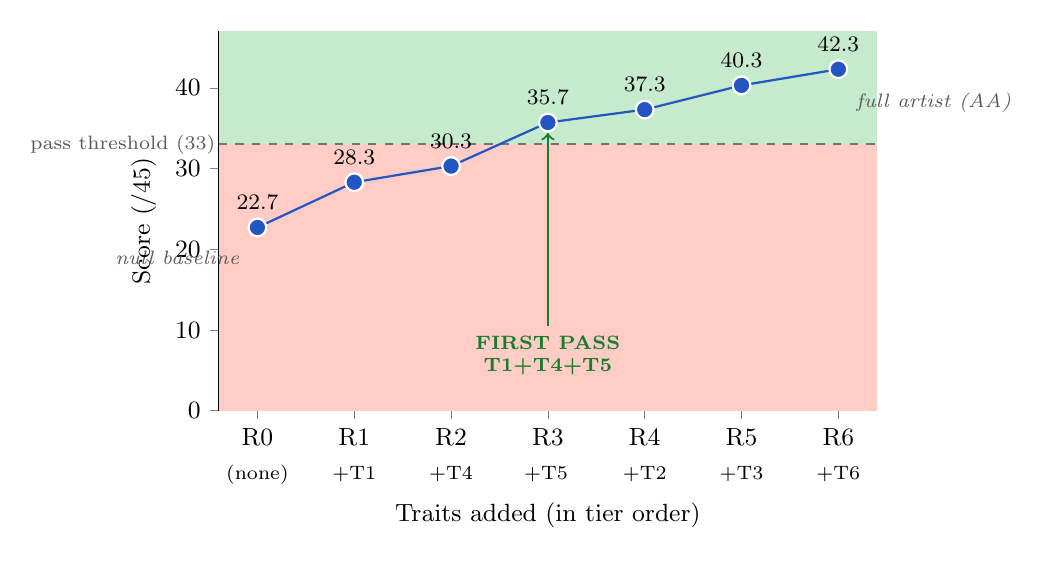
\begin{tikzpicture}
\begin{axis}[
  width=0.82\linewidth,
  height=6.4cm,
  xmin=-0.4, xmax=6.4,
  ymin=0, ymax=47,
  xlabel={Traits added (in tier order)},
  xlabel style={font=\small},
  ylabel={Score (/45)},
  ylabel style={font=\small},
  xtick={0,1,2,3,4,5,6},
  xticklabels={
    R0\\[0.3ex]{\scriptsize(none)},
    R1\\[0.3ex]{\scriptsize$+$T1},
    R2\\[0.3ex]{\scriptsize$+$T4},
    R3\\[0.3ex]{\scriptsize$+$T5\,$\bigstar$},
    R4\\[0.3ex]{\scriptsize$+$T2},
    R5\\[0.3ex]{\scriptsize$+$T3},
    R6\\[0.3ex]{\scriptsize$+$T6}
  },
  xticklabel style={font=\small, align=center},
  ytick={0,10,20,30,40},
  yticklabel style={font=\small},
  tick align=outside,
  major tick length=3pt,
  axis line style={thin},
  axis lines*=left,
  clip=false,
  enlargelimits=false,
]

  %% -------------------------------------------------------
  %% Background: FAIL region  (0 <= y <= 33), drawn as filled rectangle
  %% Use \fill in tikz coordinate space via axis cs
  %% -------------------------------------------------------
  \fill[
    fill={rgb,255:red,255;green,205;blue,198},
    draw=none,
  ]
    (axis cs:-0.4, 0) rectangle (axis cs:6.4, 33);

  %% -------------------------------------------------------
  %% Background: PASS region  (33 <= y <= 47)
  %% -------------------------------------------------------
  \fill[
    fill={rgb,255:red,198;green,235;blue,204},
    draw=none,
  ]
    (axis cs:-0.4, 33) rectangle (axis cs:6.4, 47);

  %% -------------------------------------------------------
  %% Pass threshold dashed horizontal line at y=33
  %% -------------------------------------------------------
  \addplot[
    color=black!55,
    dashed,
    thick,
    mark=none,
    forget plot,
  ] coordinates { (-0.4, 33) (6.4, 33) };

  \node[
    font=\scriptsize,
    anchor=east,
    text=black!65,
    fill=white,
    inner sep=1pt,
  ] at (axis cs: -0.4, 33) {pass threshold (33)};

  %% -------------------------------------------------------
  %% Reconstruction line: blue, filled circle markers
  %% -------------------------------------------------------
  \addplot[
    color={rgb,255:red,35;green,85;blue,195},
    thick,
    mark=*,
    mark size=3.2pt,
    mark options={
      fill={rgb,255:red,35;green,85;blue,195},
      draw=white,
      line width=0.8pt,
    },
    forget plot,
  ] coordinates {
    (0, 22.7)   % R0  null baseline
    (1, 28.3)   % R1  +T1
    (2, 30.3)   % R2  +T4
    (3, 35.7)   % R3  first pass  *** FIRST PASS ***
    (4, 37.3)   % R4  +T2
    (5, 40.3)   % R5  +T3
    (6, 42.3)   % R6  full artist
  };

  %% -------------------------------------------------------
  %% Score labels above each data point
  %% -------------------------------------------------------
  \node[font=\footnotesize, anchor=south, yshift=3pt]
    at (axis cs: 0, 22.7) {22.7};
  \node[font=\footnotesize, anchor=south, yshift=3pt]
    at (axis cs: 1, 28.3) {28.3};
  \node[font=\footnotesize, anchor=south, yshift=3pt]
    at (axis cs: 2, 30.3) {30.3};
  \node[font=\footnotesize, anchor=south, yshift=3pt]
    at (axis cs: 3, 35.7) {35.7};
  \node[font=\footnotesize, anchor=south, yshift=3pt]
    at (axis cs: 4, 37.3) {37.3};
  \node[font=\footnotesize, anchor=south, yshift=3pt]
    at (axis cs: 5, 40.3) {40.3};
  \node[font=\footnotesize, anchor=south, yshift=3pt]
    at (axis cs: 6, 42.3) {42.3};

  %% -------------------------------------------------------
  %% Annotation: "null baseline" at R0
  %% -------------------------------------------------------
  \node[
    font=\scriptsize\itshape,
    anchor=north east,
    text=black!65,
    xshift=-3pt,
    yshift=-5pt,
  ] at (axis cs: 0, 22.7) {null baseline};

  %% -------------------------------------------------------
  %% Annotation: "full artist (AA)" at R6
  %% -------------------------------------------------------
  \node[
    font=\scriptsize\itshape,
    anchor=north west,
    text=black!65,
    xshift=3pt,
    yshift=-5pt,
  ] at (axis cs: 6, 42.3) {full artist (AA)};

  %% -------------------------------------------------------
  %% Annotation: "FIRST PASS — T1+T4+T5" at R3
  %% Upward arrow from y=10 to just below the R3 data point
  %% -------------------------------------------------------
  \draw[
    ->,
    thick,
    color={rgb,255:red,25;green,125;blue,45},
  ] (axis cs: 3, 10.5) -- (axis cs: 3, 34.4);

  \node[
    font=\scriptsize\bfseries,
    anchor=north,
    text={rgb,255:red,25;green,125;blue,45},
    align=center,
    inner sep=2pt,
  ] at (axis cs: 3, 10.0) {FIRST PASS\\T1+T4+T5};

\end{axis}
\end{tikzpicture}

\caption{Reconstruction curve (Phase~3): cumulative score as traits are added
  in tier order. The quality threshold is first crossed at R3
  (T1+T4+T5 = 35.7/45, $\bigstar$). Each subsequent trait adds
  1.6--5.4 points. The minimum sufficient set is T1 + T4 + T5.}
\label{fig:reconstruction}
\end{figure}
